% !Tex root = vaje.tex
\chapter{Eksponentna in logaritemska funkcija}
\label{cha:exp-log}

\section{Pregled snovi}
\label{sec:exp-log-pregled-snovi}


\begin{center}
EKSPONENTNA FUNKCIJA
\end{center}

Eksponentna funkcija je preslikava $f: \mathbb{R} \longrightarrow \mathbb{R}^+$ oz. $f: x \longmapsto a^x \Leftrightarrow f(x) =~a^x$, pri čemer je $a > 0$ in $a \neq 1$, saj če bi bil $a=1$, bi dobili konstantno funkcijo	$f(x) = 1^x = 1$.
\\

\noindent Ločimo dva primera:
\begin{enumerate}
\item $a > 1$:
%
\begin{itemize}
\item Definicijsko območje so vsa realna števila: $\mathcal{D}_f = \mathbb{R}$.
\item Zaloga vrednosti so vsa pozitivna realna števila: $\mathcal{Z}_f = \mathbb{R}^+$.
\item Abscisna os je vodoravna asimptota, saj se približuje $y = 0$, vendar se je nikoli ne dotakne, ko gre $x \rightarrow -\infty$.
\item Začetna vrednost je pri vseh grafih enaka: $T(0,1)$, saj je $f(0) = a^0 = 1~\forall a$.
\item Funkcija je naraščajoča: $x_1 < x_2 \Rightarrow f(x_1) < f(x_2)$
\item Funkcija je injektivna: $x_1 \neq x_2 \Rightarrow f(x_1) \neq f(x_2)~\forall x_{1, 2} \in \mathbb{R}$.

%
\begin{figure}[h!]
\centering
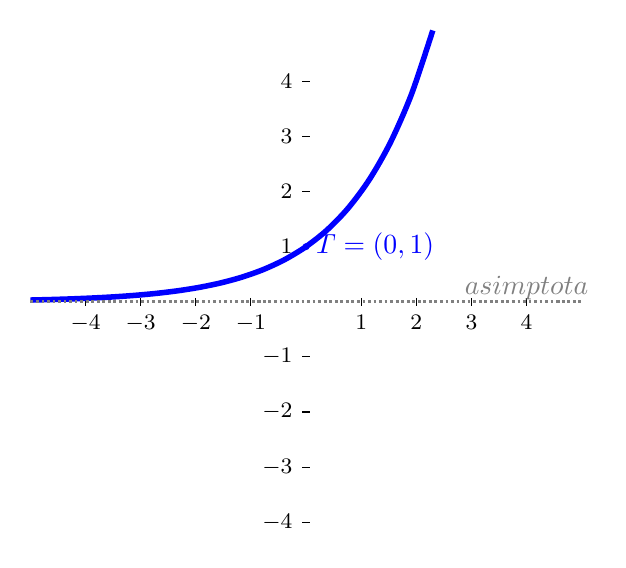
\begin{tikzpicture}[>=latex, scale=0.7]
\koordinate{-5}{5}{-5}{5}
\foreach \x in {-4,...,-1,1,2,...,4}
\draw[shift={(\x,0)}] (0pt,2pt) -- (0pt,-2pt) node[below] {\footnotesize $\x$};
\foreach \y in {-4,...,-1,1,2,...,4}
\draw[shift={(0,\y)}] (2pt,0pt) -- (-2pt,0pt) node[left] {\footnotesize $\y$};
\draw[line width=2.pt,color=blue,smooth,samples=20,domain=-5:2.3] plot(\x,{2.0^((\x))});
\draw [line width=1.pt,dash pattern=on 1pt off 1pt,color=gray,domain=-5:5] plot(\x,{(-0.-0.*\x)/1.});
\draw[color=blue] (0,1) circle (1.5pt) node[right]{$T = (0, 1)$};
\draw[color=gray] (4,0.25) node {$asimptota$};
\end{tikzpicture}
\caption{Graf, ko $a>1$}
\end{figure}
\end{itemize}
%
\newpage
\item $0 < a < 1$:
\begin{itemize}
\item $\mathcal{D}_f = \mathbb{R}$
\item $\mathcal{Z}_f = \mathbb{R}^+$
\item Abscisna os je vodoravna asimptota, saj se približuje $y = 0$, vendar se je nikoli ne dotakne, ko gre $x \rightarrow \infty$.
\item Začetna vrednost: $T(0,1)$
\item Funkcija je padajoča: $x_1 < x_2 \Rightarrow f(x_1) > f(x_2)$
\item Funkcija je injektivna.
%
\begin{figure}[h!]
\centering
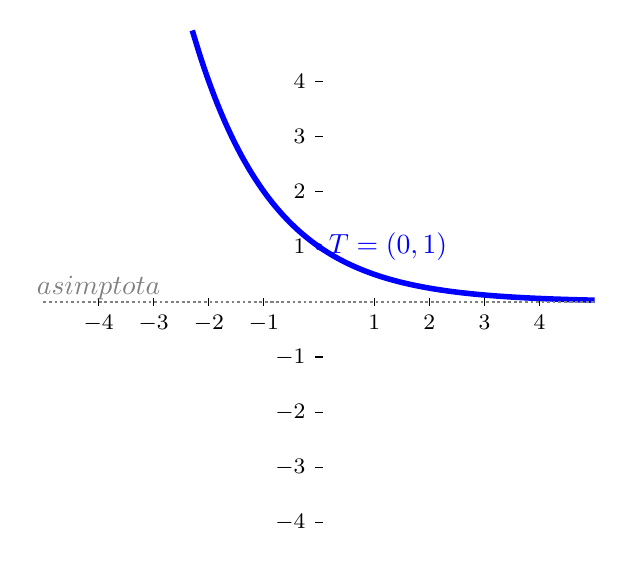
\begin{tikzpicture}[>=latex, scale=0.7]
\koordinate{-5}{5}{-5}{5}
\foreach \x in {-4,...,-1,1,2,...,4}
\draw[shift={(\x,0)}] (0pt,2pt) -- (0pt,-2pt) node[below] {\footnotesize $\x$};
\foreach \y in {-4,...,-1,1,2,...,4}
\draw[shift={(0,\y)}] (2pt,0pt) -- (-2pt,0pt) node[left] {\footnotesize $\y$};
\draw[line width=2.pt,color=blue,smooth,samples=50,domain=-2.3:5] plot(\x,{0.5^((\x))});
\draw [line width=1.pt,dash pattern=on 1pt off 1pt,color=gray,domain=-5:5] plot(\x,{(-0.-0.*\x)/1.});
\draw[color=blue] (0,1) circle (1.5pt) node[right]{$T = (0, 1)$};
\draw[color=gray] (-4,0.25) node {$asimptota$};
\end{tikzpicture}
\caption{Graf, ko $0<a<1$}
\end{figure}
\end{itemize}
\end{enumerate}
%
\newpage
\begin{zgled}
Nariši graf: $f(x) = 2^{x+1} - 3$. \\
Splošna enačba eksponetnih funkcij je: $f(x) = a^{x-p} + q$, kjer je $\vec{r}=(p, q)$ vektor premika. Koordinata $p$ bo premikala v smeri $x$-osi, $q$ pa v smeri $y$-osi. Najprej določimo osnovno eksponentno funkcijo brez premikov, ki jo bomo označili $y'=2^x$ ter vektor premika, ki je v našem primeru $\vec{r}=(-1, -3)$. Paziti moramo na predznak pri $p$, saj je v vektorju zapisan s pozitivnim predznakom, v splošni enačbi pa z negativnim predznakom. Najprej narišemo funkcijo $y'$. Narišemo jo tako, da izračunamo dve ali tri točke z grafa. Pri $x=0$ imamo vrednost 1 (svetlo zelena točka), pri $x=1$ pa vrednost 2 (siva točka). Sedaj imamo graf $y'$. Nato graf premaknemo za vektor $\vec{r}$. Ker ima prva komponenta $p$ vrednost -1, premaknemo graf za eno enoto levo (če bi imeli plus, bi se premaknili v desno) v smeri $x$-osi. Druga komponenta, komponenta $q$, pa ima vrednost -3, zato graf premaknemo v levo (če bi imeli plus, bi se premaknili v desno) za tri enote v smeri $y$-osi. Dobimo graf iskane funkcije $f(x)$.
%
\begin{figure}[h!]
\centering
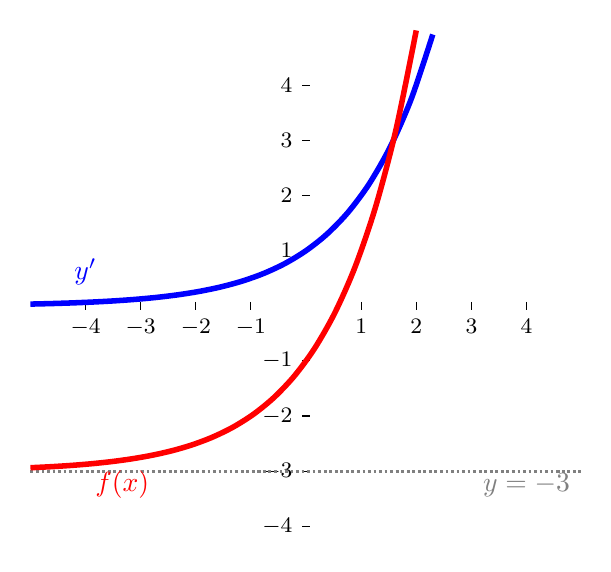
\begin{tikzpicture}[>=latex, scale=0.7]
\koordinate{-5}{5}{-5}{5}
\foreach \x in {-4,...,-1,1,2,...,4}
\draw[shift={(\x,0)}] (0pt,2pt) -- (0pt,-2pt) node[below] {\footnotesize $\x$};
\foreach \y in {-4,...,-1,1,2,...,4}
\draw[shift={(0,\y)}] (2pt,0pt) -- (-2pt,0pt) node[left] {\footnotesize $\y$};
\draw[line width=2.pt,color=blue,smooth,samples=20,domain=-5:2.3] plot(\x,{2.0^((\x))});
\draw [line width=1.pt,dash pattern=on 1pt off 1pt,color=gray,domain=-5:5] plot(\x,{(-3.-0.*\x)/1.});
\draw[line width=2.pt,color=red,smooth,samples=20,domain=-5:2] plot(\x,{2.0^((\x)+1.0)-3.0});
\draw[color=blue] (-4, 0.2) node[above]{$y'$};
\draw[color=red] (-4, -3.25) node[right]{$f(x)$};
\draw[color=gray] (4,-3.25) node {$y=-3$};
\end{tikzpicture}
\end{figure}
%
\end{zgled}

\newpage
\begin{center}
EKSPONENTNE ENAČBE
\end{center}

Eksponente enačbe so enačbe, ki imajo neznanke le v eksponentu. Najprej si osvežimo spomin, kako se računa s potencami:
$x, z \in \mathbb{R}, a, b > 0, a, b \neq 1$:
%
\begin{multicols}{2}
\begin{itemize}
\item $a^x \cdot a^z = a^{x + z}$
\item $a^x : a^z = a^{x - z}$
\item $(a^x)^z = a^{x\cdot z}$
\item $a^x \cdot b^x = (a \cdot b)^x$
\item $\frac{a^x}{b^x} = (\frac{a}{b})^x$
\item $a^{-x} = \frac{1}{a^x}$
\item $a^0 = 1, a\neq 0$
\item$a^1 = a$
\item $a^{\frac{p}{q}} = \sqrt [q]a^p$
\item $(\sqrt[q]a^p)^n = \sqrt[q]{a^{np}}$
\end{itemize}
\end{multicols}

Eksponentne enačbe ločimo v pet skupin:
%
\begin{enumerate}
\item \textbf{osnovi potenc na obeh straneh enačbe sta enaki} oz. enačbo preuredimo tako, da imamo na obeh straneh enaki osnovi: $a^{f(x)} = a^{g(x)}$. Enačaj bo veljal le, če bosta eksponenta enaka: $f(x) = g(x)$.
%
\begin{zgled}
Reši enačbo: $2^{x+3} = 4^{3x+1}$.
\begin{align*}
\intertext{Najprej enačbo preuredimo, da bomo imeli na obeh straneh enaki osnovo:}
2^{x+3} &= (2^2)^{3x-1}\\
\intertext{Uporabimo pravilo $(a^x)^z = a^{x\cdot z}$:}\\
2^{x+3} &= (2)^{6x-2}
\intertext{Eksponenta morata biti enaka, da bo leva stran enačbe enaka desni:}
x+3 &= 6x-2
\intertext{Ven izračunamo $x$:}
x&=1
\end{align*}
\end{zgled}
%
\item \textbf{potenci imata različni osnovi, vendar enak eksponent:} $a^{f(x)} =b^{f(x)}$. Enačaj bo v tem primeru veljal le, če bosta eksponenta enaka nič, saj grafa eksponentne funkcije z različnima osnovama potekata skozi eno skupno točko in sicer $T(0, 1) \Rightarrow f(x) = 0$ (glej \ref{fig: grafa}) ali:
%
\begin{equation*}
\bigg(\frac{a}{b}\bigg)^{f(x)}=1 \Rightarrow \bigg(\frac{a}{b}\bigg)^{f(x)} = \bigg(\frac{a}{b}\bigg)^0 \text{po zgornji točki}\Rightarrow f(x) = 0.
\end{equation*}
%
\begin{figure}[h!]
\centering
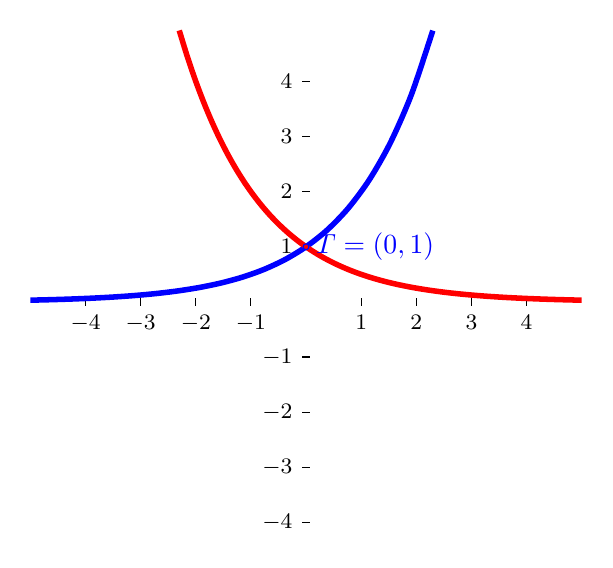
\begin{tikzpicture}[>=latex, scale=0.7]
\koordinate{-5}{5}{-5}{5}
\foreach \x in {-4,...,-1,1,2,...,4}
\draw[shift={(\x,0)}] (0pt,2pt) -- (0pt,-2pt) node[below] {\footnotesize $\x$};
\foreach \y in {-4,...,-1,1,2,...,4}
\draw[shift={(0,\y)}] (2pt,0pt) -- (-2pt,0pt) node[left] {\footnotesize $\y$};
\draw[line width=2.pt,color=blue,smooth,samples=20,domain=-5:2.3] plot(\x,{2.0^((\x))});
\draw[line width=2.pt,color=red,smooth,samples=50,domain=-2.3:5] plot(\x,{0.5^((\x))});
\draw[color=blue] (0,1) circle (1.5pt) node[right]{$T = (0, 1)$};
\end{tikzpicture}
\caption{Grafa dveh eksponentnih funkcij}
\label{fig: grafa}
\end{figure}
\\
\begin{zgled}
Reši enačbo: $5^{x-1} = 4^{x-1}$.
\begin{align*}
\intertext{Enačaj bo veljal le v primeru, ko bo eksponent enak 0:}
x-1&=0
\intertext{Izrazimo $x$:}
x&=1
\end{align*}
\end{zgled}
%
\item \textbf{neznanka v eksponentu potence je pomnožena z različnimi koeficienti:} $a^{bx + c}$. Enačbo poenostaviš tako, da vpelješ novo spremenljivko $u$, kjer bo eksponent najmanjši faktor ter računaš naprej kvadratno enačbo z $u$-ji.
%
\begin{zgled}
Reši enačbo: $2^x+2^{2x-1=4}.$
\begin{align*}
\intertext{Uporabimo pravilo $a^x \cdot a^z = a^{x + z}$:}
2^x+2^{2x}\cdot 2^{-1}&=4
\intertext{Vpeljemo novo spremenljivko u, za katero vzamemo najmanjši faktor: $u=2^x$ ter zapišemo prenovljeno enačbo:}
u+u^2\cdot\frac{1}{2}&=4
\intertext{Množimo z 2, da se znebimo ulomka in dobimo kvadratno enačbo:}
u^2+2u-8&=0
\intertext{Razcepimo po Vietovem pravilu:}
(u-2)(u+4)&=0
\intertext{Dobimo dve rešitvi: $u_1=2$ in $u_2=-4$ ter pogledamo kaj je bil u. V prvem primeru dobimo $2=2^x \Rightarrow x=1$, v drugem pa $-4=2^x$, kar pa ne more biti enako, saj je 2 na neko potenco vedno pozitivno število.}
\end{align*}
\end{zgled}
%
\item \textbf{enačbe, kjer nastopajo eksponentne in neeksponentne funkcije:} $a^{f(x)} = b$, kjer $b$ ni potenca števila $a$ ali $a^{f(x)} = x + c$. V takem primeru najprej narišemo grafa obeh funkcij, ki ju vsebuje enačba. Z grafa prebereš rešitve. 
%
\begin{zgled}
Reši enačbo: $3^x=1-x$.\\
Narišemo grafa funkcij $f(x)=3^x$ in $g(x)=1-x$ in pogledamo kje se sekata, saj imata v presečišču oba grafa enako vrednost.
%
\begin{figure}[h!]
\centering
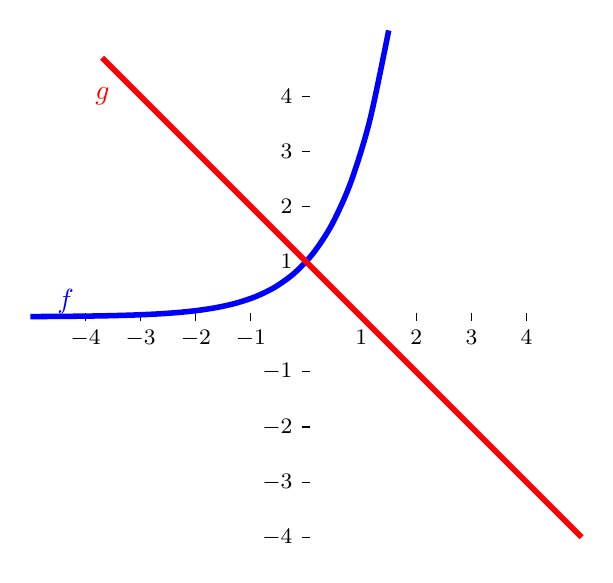
\begin{tikzpicture}[>=latex, scale=0.7]
\koordinate{-5}{5}{-5}{5}
\foreach \x in {-4,...,-1,1,2,...,4}
\draw[shift={(\x,0)}] (0pt,2pt) -- (0pt,-2pt) node[below] {\footnotesize $\x$};
\foreach \y in {-4,...,-1,1,2,...,4}
\draw[shift={(0,\y)}] (2pt,0pt) -- (-2pt,0pt) node[left] {\footnotesize $\y$};
\draw[line width=2.pt,color=blue,smooth,samples=20,domain=-5:1.5] plot(\x,{3.0^((\x))});
\draw[line width=2.pt,color=red,smooth,samples=50,domain=-3.7:5] plot(\x,{1.0-(\x)});
\draw[color=blue] (-4.36223082314358,0.2813862402325262) node {$f$};
\draw[color=red] (-4,4) node[right] {$g$};
\end{tikzpicture}
\caption{Grafično reševanje enačb}
\end{figure}
%
Neodvisna spremenljivka $x$ v presečišču je kandidat za rešitev. V našem primeru: $x=0$. Preverimo ali je $x=0$ res rešitev in sicer tako, da ga vstavimo nazaj v obe strani enačbe in dobimo: $3^0=1$ in $1-0=1 \Rightarrow$ rešitev je $x=0$.
\end{zgled}
%
\item \textbf{enačbe, kjer nastopajo vsote ali razlike potenc z enakimi osnovami} rešujemo  z izpostavljanjem skupnega faktorja. Tako enačbo prevedemo na že znane eksponntne enačbe.
%
\begin{zgled}
Reši enačbo: $2^{x-4}+3 \cdot 2^{x-2} - 2^{x-1} = 20$.
\begin{align*}
\intertext{Izpostavimo najmanjši skupni faktor:}
2^{x-4}(1+3\cdot2^2-2^3)&=20
\intertext{Poračunamo oklepaj:}
2^{x-4}\cdot5 &= 20
\intertext{Delimo s 5:}
2^{x-4}&=4
\intertext{Preoblikujemo, da bomo imeli na obeh straneh enako osnovo:}
2^{x-4}&=2^2
\intertext{Enačimo eksponente in dobimo:}
x-4&=2 \Rightarrow x=6
\end{align*}
\end{zgled}
\end{enumerate}

\begin{center}
EKSPONENTNE NEENAČBE
\end{center}
Eksponentne neenačbe so podobne eksponetnim enačbam, le da imajo vmes neenačaj. Rešitve neenačb so intervali, unije intervalov ali prazna množica. Prav tako kot pri eksponentnih enačbah lahko rešujemo neenačbe na različne načine:
%
\begin{enumerate}
\item \textbf{osnovi potenc na obeh straneh neenačbe sta enaki in $a>1$} oz. neenačbo preuredimo tako, da imamo na obeh straneh enaki osnovi: $a^{x_1} > a^{x_2} \Rightarrow x_1 > x_2$.
%
\begin{zgled}
Reši neenačbo: $4^{x-1} > 0,5^{3x+2}$.
\begin{align*}
\intertext{Prevedemo neenačbo, da imamo na obeh straneh enaki osnovi:}
2^{2x-2} &> 2^{-3x-2}
\intertext{Ker sta osnovi enaki nas zanimajo le še eksponenti:}
2x-2&>-3x-2
\intertext{Uredimo in dobimo:}
5x &> 0 \Rightarrow x>0
\end{align*}
\end{zgled}
%
\item \textbf{potenci imata različni osnovi, vendar enak eksponent in $a>1$:} $a^x < b^x$. Delimo neenačbo s tisto potenco, ki ima manjšo osnovo.
%
\begin{zgled}
Reši neenačbo: $2^x < 3^x$.
\begin{align*}
\intertext{Neenačbo delimo z $2^x$, saj ima manjšo osnovo:}
1&<\frac{3^x}{2^x}
\intertext{Na desni strani uporabimo pravilo: $\frac{a^x}{b^x} =(\frac{a}{b})^x$, na levi pa: $a^0 = 1$:}
\Big(\frac{3}{2}\Big)^0 &< \Big(\frac{3}{2}\Big)^x
\intertext{Dobimo rešitev:}
x&>0
\end{align*}
\end{zgled}
%
\item \textbf{osnovi potenc na obeh straneh enačbe sta enaki in $0<a<1$:}
\\
$a^{x_1}<a^{x_2} \Rightarrow x_1 > x_2$.
%
\begin{zgled}
Reši neenačbo: $0,01^{3x}<0,0001^{1+2x}$.
\begin{align*}
\intertext{Preoblikujemo tako, da imamo na obeh straneh enki osnovi:}
0,01^{3x} &< 0,01^{2+4x}
\intertext{Ko gledamo eksponente se neenačaj obrne, ker imamo osnovo med 0 in 1:}
3x&>2+4x
\intertext{Dobimo rešitev:}
x&<-2
\end{align*}
\end{zgled}
%
\end{enumerate}

\begin{center}
LOGARITEMSKA FUNKCIJA
\end{center}

Ker je eksponentna funkcija  $f: x \mapsto a^x$ bijektivna, je obrnljiva, kar pa pomeni, da ima inverz $f^{-1}$. Njena inverzna funkcija je logaritemska funkcija z enako osnovo. Logaritemska funkcija z osnovo $a$, kjer je $a > 0$ in $a \neq 1$ je preslikava $f: x \mapsto \log_a{x}$, za vse $x > 0$, pri čemer je $x$ argument logaritma. Torej velja:
\begin{equation*}
a^x=y \Leftrightarrow x=\log_a{y}
\end{equation*}
%
Iz te definicije sledi tudi: 
\begin{equation*}
a^{\log_a{y}} = y \qquad \text{in} \qquad \log_a{a^x} = x
\end{equation*}
%
Gaf logaritemske funkcije dobimo tako, da čez simetralo lihih kvadrantov $y=x$ prezrcalimo eksponentno funkcijo, saj je njen inverz. Tako kot pri eksponentni funkciji tudi tu ločimo dva preimera:
\begin{enumerate}
\item $a>1$:
%
\begin{itemize}
\item  $\mathcal{D}_f = \mathbb{R}^+$
\item $\mathcal{Z}_f = \mathbb{R}$
\item Ordinatna os je navpična asimptota.
\item Vsi grafi gredo skozi točko $T(1, 0)$, saj je ena ničla logaritma: $\log_a{1}=\log_a{a^0}
=0$.
\item Funkcija je naraščajoča: $x_1 < x_2 \Rightarrow f(x_1) < f(x_2)$
\item Funkcija je neomejena: ko vrednosti spremenljivke $x$ naraščajo od $-\infty$ do $+\infty$, graf funkcije narašča od minus neskončno do neskončnosti, zato funkcija navzdol in navzgor ni omejena.
\item Funkcija je pozitivna na intervalu $(1, \infty)$ in negativna na $(0, 1)$.
%
\begin{figure}[h!]
\centering
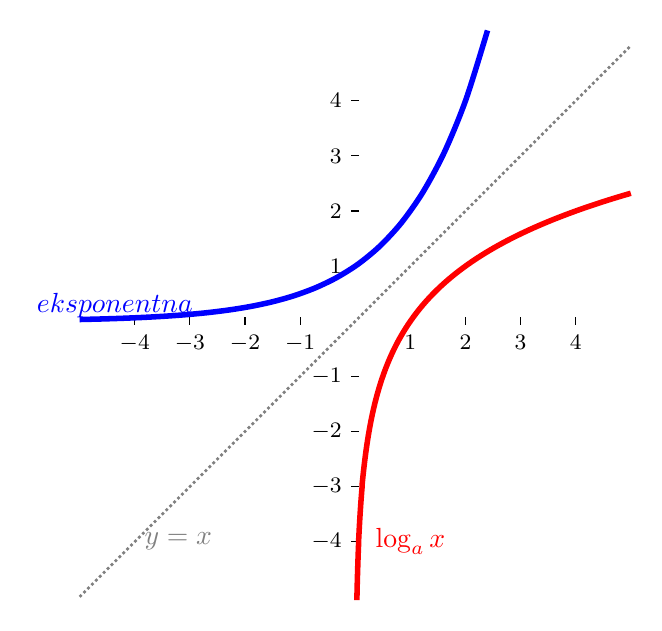
\begin{tikzpicture}[>=latex, scale=0.7]
\koordinate{-5}{5}{-5}{5}
\foreach \x in {-4,...,-1,1,2,...,4}
\draw[shift={(\x,0)}] (0pt,2pt) -- (0pt,-2pt) node[below] {\footnotesize $\x$};
\foreach \y in {-4,...,-1,1,2,...,4}
\draw[shift={(0,\y)}] (2pt,0pt) -- (-2pt,0pt) node[left] {\footnotesize $\y$};
\draw[line width=2.pt,color=blue,smooth,samples=20,domain=-5:2.4] plot(\x,{2.0^((\x))});
\draw[line width=1.pt,color=gray,dash pattern=on 1pt off 1pt,samples=50,domain=-5:5] plot(\x,{0.0(\x)});
\draw[line width=2.pt,color=red,smooth,samples=4001,domain=0.03:5] plot(\x,{log2(\x)});
\draw[color=blue] (-4.36223082314358,0.2813862402325262) node {$eksponentna$};
\draw[color=gray] (-4,-4) node[right] {$y=x$};
\draw[color=red] (1,-4) node {$\log_a{x}$};
\end{tikzpicture}
\caption{Graf logaritma $a>1$}
\label{fig: graf osnove več od 1}
\end{figure}
\end{itemize}

\item $0 < a < 1$:
%
\begin{itemize}
\item  $\mathcal{D}_f = \mathbb{R}^+$
\item $\mathcal{Z}_f = \mathbb{R}$
\item Ordinatna os je navpična asimptota.
\item Vsi grafi gredo skozi točko $T(1, 0)$, saj je ena ničla logaritma: $\log_a{1}=0$.
\item Funkcija je padajoča: $x_1 < x_2 \Rightarrow f(x_1) > f(x_2)$
\item Funkcija je neomejena.
\item Funkcija je negativna na intervalu $(1, \infty)$ in pozitivna na $(0, 1)$.
%
\begin{figure}[h!]
\centering
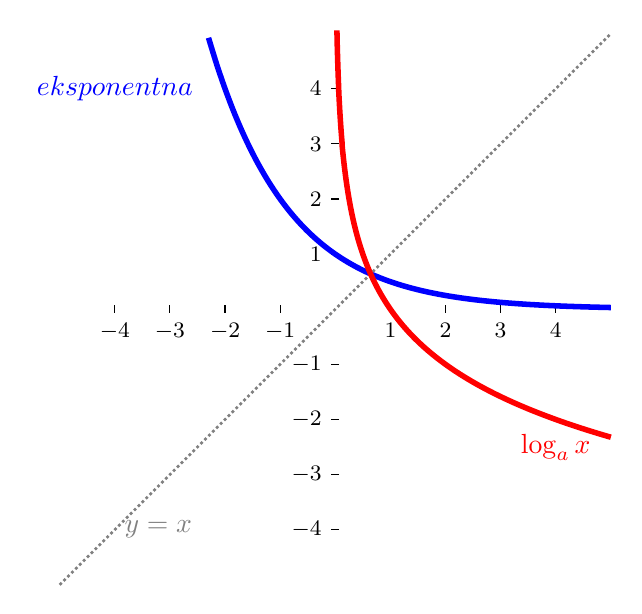
\begin{tikzpicture}[>=latex, scale=0.7]
\koordinate{-5}{5}{-5}{5}
\foreach \x in {-4,...,-1,1,2,...,4}
\draw[shift={(\x,0)}] (0pt,2pt) -- (0pt,-2pt) node[below] {\footnotesize $\x$};
\foreach \y in {-4,...,-1,1,2,...,4}
\draw[shift={(0,\y)}] (2pt,0pt) -- (-2pt,0pt) node[left] {\footnotesize $\y$};
\draw[line width=2.pt,color=blue,smooth,samples=50,domain=-2.3:5] plot(\x,{0.5^((\x))});
\draw[line width=1.pt,color=gray,dash pattern=on 1pt off 1pt,samples=50,domain=-5:5] plot(\x,{0.0(\x)});
\draw[line width=2.pt,color=red,smooth,samples=4001,domain=0.03:5] plot(\x,{ln((\x))/ln(0.5)});
\draw[color=blue] (-4,4) node {$eksponentna$};
\draw[color=gray] (-4,-4) node[right] {$y=x$};
\draw[color=red] (4,-2.5) node {$\log_a{x}$};
\end{tikzpicture}
\end{figure}
\end{itemize}
\end{enumerate}

\begin{zgled}
Nariši graf funkcije: $f(x) = \log_2{(2x)}+1$.
\begin{align*}
\intertext{Tako kot pri eksponentni funkciji najprej določimo osnovno funkcijo. Osnovna funkcija bo sedaj vsebovala le logaritem brez premikov po $y$-osi in brez zrcaljenja: $y' = \log_2{(2x)}$. Nato funkcijo $y'$ narišemo v treh korakih:}
\intertext{1) Poiščemo definicijsko območje tako, da upoštevamo pogoj: argument je večji od 0. Torej:}
2x&>0
\intertext{Iz tega sledi:}
x&>0
\intertext{Narišemo navpično asimptoto pri $x=0$. Ker smo izračunali, da je ta logaritem definiran le za tiste $x$, ki so večji od $0$, bo naš graf na desni strani narisane asimptote.} 
\intertext{2) Poiščemo ničlo. Logaritemske funkcije imajo ničlo, ko je argument enak 1. Torej:}
2x=1 \Rightarrow x=\frac{1}{2}
\intertext{Narišemo ničlo.}
\intertext{3) Izračunamo točko, kjer ima logaritem vrednost 1. To bo takrat, ko bo argument enak osnovi logaritma:}
2x = 2 \Rightarrow x=1
\intertext{Narišemo torej točko $T(1, 1)$. Čez dobljeni točki narišemo graf logaritemske funkcije. Tako smo dobili graf $y'$. Graf $y'$ je potrebno še premakniti v smeri $y$-osi. Logaritmu je prišteta enka, zato narisan graf prestavimo za eno enoto v desno (če bi enko odšteli, bi s prestavili za eno enoto v levo) in dobimo željeno funkcijo $f(x)$.}
\end{align*}

\begin{figure}[h!]
\centering
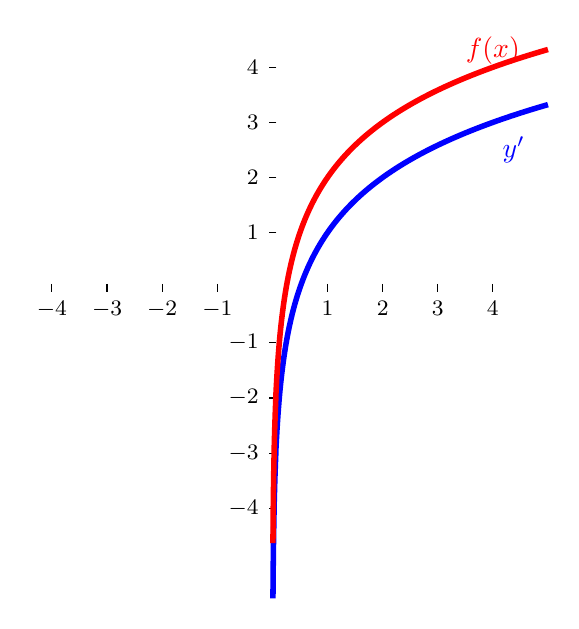
\begin{tikzpicture}[>=latex, scale=0.7]
\koordinate{-5}{5}{-5}{5}
\foreach \x in {-4,...,-1,1,2,...,4}
\draw[shift={(\x,0)}] (0pt,2pt) -- (0pt,-2pt) node[below] {\footnotesize $\x$};
\foreach \y in {-4,...,-1,1,2,...,4}
\draw[shift={(0,\y)}] (2pt,0pt) -- (-2pt,0pt) node[left] {\footnotesize $\y$};
\draw[line width=2.pt,color=blue,smooth,samples=4001,domain=0.01:5] plot(\x,{ln(2.0*(\x))/ln(2.0)}););
\draw[line width=2.pt,color=red,smooth,samples=4001,domain=0.01:5] plot(\x,{ln(2.0*(\x))/ln(2.0)+1}););
\draw[color=blue] (4,2.5) node[right] {$y'$};
\draw[color=red] (4,4.3) node {$f(x)$};
\end{tikzpicture}
\end{figure}
%
\end{zgled}

Za računanje z logaritmi velja nekaj pravil:
\begin{multicols}{2}
\begin{itemize}
\item $y=a^x \Rightarrow x=\log_a{y}$
\item $\log_a{a^x} = x$
\item $\log_a{a}=1$
\item $\log_a{1}=0$
\item$a^{\log_a{y}}=y$
\item $\log_a{(x\cdot z)}=\log_a{x} + \log_a{z}$
\item $\log_a{x^r}=r \cdot \log_a{x}; \qquad r \in \mathbb{R}$
\item $\log_a{(\frac{x}{z})}=\log_a{x}-\log_a{z}$
\item $\log_a{x}=\frac{\log_b{x}}{\log_b{a}}$
\end{itemize}
\end{multicols}

V matematiki največ uporabljamo logaritma z osnovo 10, ki mu pravimo desetiški logaritem in logaritem z osnovo $e$, ki ga imenujemo naravni logaritem. Po dogovoru pišemo:
%
\begin{equation*}
\log_{10}{x} = \log{x} \qquad \text{in} \qquad \log_e{x} = \ln x
\end{equation*}

Logaritemske enačbe in neenačbe rešujemo s pravili za logaritmiranje.
\\
\begin{zgled}
Reši logaritemsko neenačbo: $\log_2{( \frac{x^2}{3}-\frac{x}{3}-2)}\geq 0$
\begin{align*}
\intertext{Če pogledamo graf logaritemske funkcije, ko je osnova večja od 1 (glej \ref{fig: graf osnove več od 1}), vidimo, da je funkcija pozitivna, ko je argument večji ali enak 1. Torej:}
\frac{x^2}{3}-\frac{x}{3}-2 &\geq 1
\intertext{Pomnožimo s 3, da se znebimo ulomkov, malo preuredimo in dobimo kvadratno enačbo:}
x^2 - x - 9 &\geq 0
\intertext{Izračunamo ničle:}
x_{1,2} &= \frac{1\pm \sqrt{37}}{2}
\intertext{Pogledamo, kje kvadratna funkcija pozitivna in dobimo rešitev:}
\mathcal{D}_f &= \Bigg(-\infty,\frac{1- \sqrt{37}}{2}\Bigg) \bigcup \Bigg(\frac{1+ \sqrt{37}}{2}, \infty\Bigg)
\end{align*}
\end{zgled}

\begin{zgled}
Reši logaritemsko enačbo: $\log_4{(5x+2)}=2$.
\begin{align*}
\intertext{Uporabimo definicijo logaritma: $a^x=y \Leftrightarrow x=\log_a{y}$ in dobimo:}
5x +2 &= 4^2
\intertext{Izračunamo ven $x$:}
x&=\frac{14}{5}
\end{align*}
\end{zgled}

\section{Vaje}
\label{sec:exp-log-vaje}

%%%%%%%%%%%%%%%%%%%%%%%%%%%%%%%%%%%%%%%%%%%%%%%%%%%%%%%%%%%%%%%%%%%%%%
% Odpremo datoteko, v katero se bodo zapisali odgovori za
% to poglavje.

% Določimo ime datoteke, v katero se bodo pisali odgovori.
% Vsako poglavje mora imeti svojo datoteko.
\def\datotekaOdgovori{odgovori-explog}

% Odpremo datoteko z odgovori.
\Opensolutionfile{odgovor}[\datotekaOdgovori]

%%%%%%%%%%%%%%%%%%%%%%%%%%%%%%%%%%%%%%%%%%%%%%%%%%%%%%%%%%%%%%%%%%%%%%
% VAJE
%
% Sem vstavimo vaje s pomočjo okolja "vaja". Odgovor napišemo v vajo,
% v okolje "odgovor".

\begin{vaja}
 Poenostavi naslednji izraz: \(\sqrt{x^{\frac{10}{3}}y^{\frac{4}{2}}}(x^{2}y^{\frac{1}{2}})^{4}\).

  \begin{odgovor}
   Vsa števila moramo najprej napisati v taki obliki, da so potence realna števila. 
	$$\sqrt{x^{\frac{10}{3}}y^{\frac{4}{2}}}(x^{2}y^{\frac{1}{2}})^{4}=(x^{\frac{10}{3}}y^{\frac{4}{2}})^{\frac{1}{2}}(x^{2}y^{\frac{1}{2}})^{4}=x^{\frac{10}{6}}yx^{8}y^{2}=y^{3}x^{\frac{29}{3}}$$
  \end{odgovor}
\end{vaja}

\begin{vaja}
  Čim bolj poenostavi naslednji izraz: \(\,x^{\frac{5}{3}}y^{\frac{8}{7}}\sqrt{\sqrt{x^{\frac{1}{7}}y^{\frac{14}{3}}}}\).

  \begin{odgovor}
   Rešitev: $x^{\frac{1}{28}} y^{\frac{97}{42}}$.
  \end{odgovor}
\end{vaja}

\begin{vaja}
  Napiši vse rešitve naslednje enačbe \( 8^m=32\).

  \begin{odgovor}
   Enačbo želimo najprej  preurediti v obliko $a^{f(x)}=b^{g(x)}$, potem pa imamo 2 različni možnosti:
	\begin{itemize}
		\item[a)] $a=b$ 

			v tem primeru velja: $a^{f(x)}=a^{g(x)}$, kar pa drži natanko tedaj, ko je $f(x)=g(x)$ saj je $a^x$ injektivna.
			
		\item[b)] $a\neq b$:
			
			v tem primeru pa velja $a^{f(x)}=b^{g(x)}$. Ker sta a in b različna, se te enačbe lotimo s pomočjo logartima.
			$$a^{f(x)}=b^{g(x)}\implies f(x)\log(a)=g(x)\log(b)$$
	\end{itemize}
	
	Ta primer je tipa a), saj :
	\begin{align*}
		8^m&=32\\
		(2^3)^m&=2^5\\
		2^{3m}&=2^5\\
		3m&=5\\
		m&=\frac{5}{3}
	\end{align*}
  \end{odgovor}
\end{vaja}


\begin{vaja}
	Določi vse rešitve za katere velja: \(3^{x^2-4x}=1/81\).
  \begin{odgovor}$x_{1,2}=2$.
  \end{odgovor}
\end{vaja}


\begin{vaja}
  Reši enačbo $4^{x-1}=3^x$.

  \begin{odgovor}
	\begin{align*}
	 4^{x-1}&=3^x\\
	 (2^2)^{x-1}&=3^x\\
	 2^{2x-2}&=3^x\\
	 (2x-2)\log(2)&=x\log(3)\\
	 2x\log2-x\log(3)&=2\log2\\
	 x(2\log2-\log3)&=2\log2\\
	 x&=\frac{2\log2}{2\log2-\log3}\\
	 x&=\frac{2\log2}{\log{\frac{4}{3}}}
	\end{align*}    
  \end{odgovor}
\end{vaja}

\begin{vaja}
	Izračunaj rešitve enačbe \( 15^{x-2}=5^x\).
  \begin{odgovor}
   	$x=2+\frac{\log25}{\log3}$
  \end{odgovor}
\end{vaja}

\begin{vaja}
	Kateri x-i zadoščajo enačbi \(-7\cdot 3^x+9^x=-12\).
  \begin{odgovor}
   	Enačbo najprej prepišemo v tako obliko, da bodo v osnovi eksponenta praštevila in poskusimo:
	\begin{align*}
	-7 \cdot 3^x+9^x&=-12\\
	-7\cdot 3^x+3^{2x}&=-12\\
	-7\cdot 3^x+(3^x)^2&=-12\quad \text{vpeljimo novo neznanko } 3^x=y\\
	-7y+y^2&=-12\\
	y^2-7y+12&=0\\
	y_{1}=4 \lor y_{2}=3 & \quad \text{pretvorimo sedaj nazaj na prvotno spremenljivko}\\
	x_{1}&=\log_{3}{4}\\
	x_{2}&=\log_{3}{3}=1
	\end{align*}
  \end{odgovor}
\end{vaja}

\begin{vaja}
	Napiši rešitve enačbe $-16 \cdot 2^x+4^x=-64$.
  \begin{odgovor}
   	x=3.
  \end{odgovor}
\end{vaja}

\begin{vaja}
Določi interval, kjer bo $e^x < 16$.
  \begin{odgovor}
   Najprej enačbo logaritmiramo z $\ln$ in dobimo:
\begin{align*}
\ln{e^x}&< \ln 16 \\
x &< \ln 16
\end{align*}
  \end{odgovor}
\end{vaja}

\begin{vaja}
Kdaj je $2^{2x} \geq 127 \cdot 2^x + 128$?
  \begin{odgovor}
   $x \geq 7$
  \end{odgovor}
\end{vaja}

\begin{vaja}
  \begin{odgovor}
   
  \end{odgovor}
\end{vaja}
%%%%%%%%%%%%%%%%%%%%%%%%%%%%%%%%%%%%%%%%%%%%%%%%%%%%%%%%%%%%%%%%%%%%%%
% Treba je zapredi datoteko z odgovori

\Closesolutionfile{odgovor}

%%%%%%%%%%%%%%%%%%%%%%%%%%%%%%%%%%%%%%%%%%%%%%%%%%%%%%%%%%%%%%%%%%%%%%
% Odgovori

\section{Odgovori}
\label{sec:explog-odgovori}

% Vključimo odgovore.
\input{\datotekaOdgovori}


%%% Local Variables:
%%% mode: latex
%%% TeX-master: "vaje"
%%% End:
